% 第 7 章 Viewing Schematics
\bichapter{查看原理图}{Viewing Schematics}
\label{chap:gui-sch}

IC Compiler II 支持设计原理图，用来查看设计中的逻辑元件（块与门）。原理图以图形显示层次单元。可以在设计层次中向上或向下，查看每一层设计的原理图。

本章包括以下主题：
\begin{itemize}
  \item 原理图视图
  \item 原理图中的 WordView
  \item 在原理图上标注属性
  \item 在原理图上添加管脚标记
\end{itemize}

\section{原理图视图}
\subsection*{Schematic View}

查看原理图：
\begin{itemize}
  \item 在主菜单或 Hierarchy Browser 中选择 \textbf{View > Schematic View}；
  \item 或单击工具栏上的原理图按钮。
\end{itemize}

原理图视图用于直观分析时序与逻辑，供后续优化使用。例如可以：
\begin{itemize}
  \item 查看设计或子设计中逻辑元件（块与门）的图形；
  \item 聚焦关键路径，检查时序问题。
\end{itemize}

要定制原理图视图，使用工具右侧选项卡中的 View Settings 面板。视图属性的保存方式见第~\ref{chap:gui-start}~章。

\begin{seeAlsoBox}
设置并保存视图属性，见第~\ref{chap:gui-start}~章。
\end{seeAlsoBox}

\section{原理图中的 WordView}
\subsection*{WordView in the Schematic View}

WordView 用宽组合逻辑门建立模型，便于在原理图中表示。对尚未映射的逻辑，WordView 让原理图更干净：工具用一个宽逻辑门代替级联门，并把总线实例显示为折叠形式。做面积估算时，WordView 能更准确地反映 RTL 中的原始逻辑。

WordView 使用 WVGTECH 库，而不是 GTECH 库。工具要推断这些门，必须能用到 WVGTECH 库。

在原理图视图中，GUI 用 WordView 门显示：
\begin{itemize}
  \item 总线实例（bused instance）
  \item 宽门（wide gate）
  \item 运算符（operator）
  \item 映射到多位单元的总线寄存器
\end{itemize}

图~\ref{fig:gui-117} 是折叠后的总线实例，这里是一个四输入的 WVGTECH\_AND。

\begin{figure}[htbp]
\centering
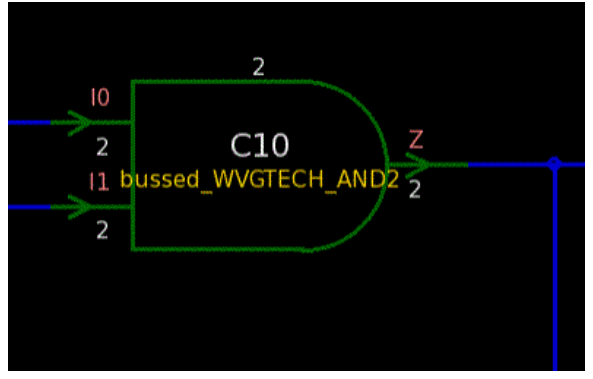
\includegraphics[width=0.72\textwidth]{gui-fig-117.png}
\caption{总线实例的折叠视图}
\label{fig:gui-117}
\end{figure}

选中 WVGTECH 门，打开上下文菜单并选择 \textbf{Expand > Selected Objects}，即可展开。默认情况下，总线实例以虚线边框显示，见图~\ref{fig:gui-118}。总线网用一条粗蓝线表示，总线反相器使用同一逻辑符号加一条粗绿线。对总线对象，可用原理图上下文菜单中的 Expand 或 Collapse 在标量表示与总线表示之间切换。

\begin{figure}[htbp]
\centering
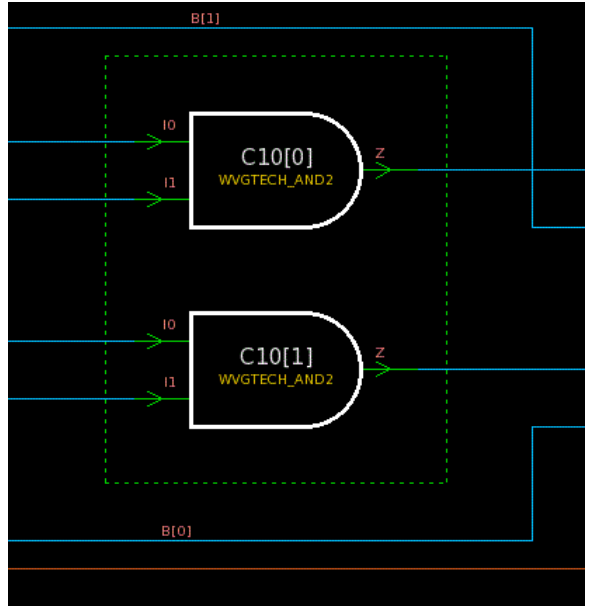
\includegraphics[width=0.72\textwidth]{gui-fig-118.png}
\caption{总线实例的展开视图}
\label{fig:gui-118}
\end{figure}

图~\ref{fig:gui-119} 是 WordView 宽门的例子。该 XOR 有 16 个输入管脚，名为 WVGTECH\_XOR16。

\begin{figure}[htbp]
\centering
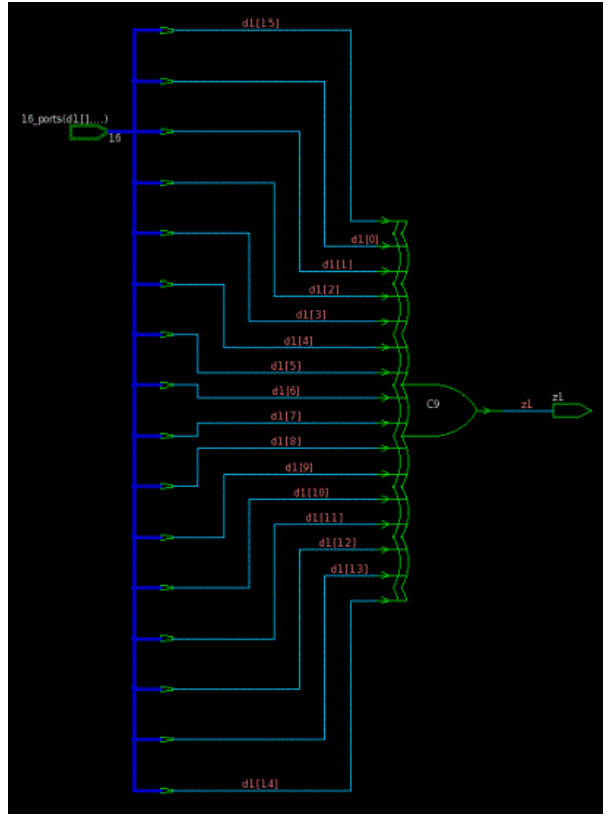
\includegraphics[width=0.55\textwidth]{gui-fig-119.png}
\caption{宽门示例}
\label{fig:gui-119}
\end{figure}

运算符在 GUI 中画成基本符号，见图~\ref{fig:gui-120}。此例表示加法运算符。

\begin{figure}[htbp]
\centering
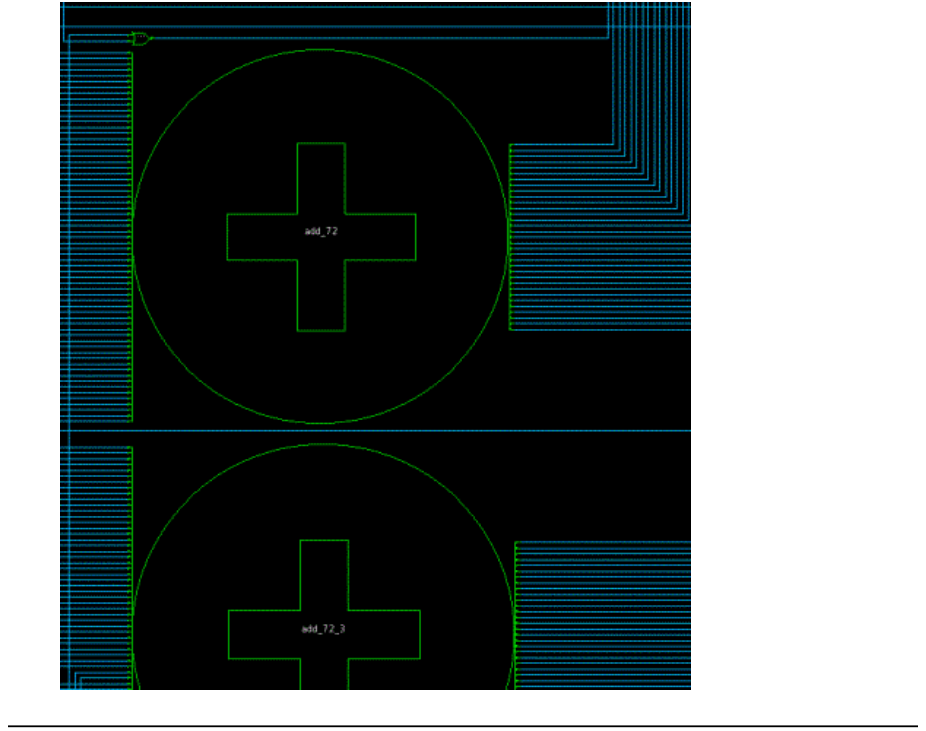
\includegraphics[width=0.45\textwidth]{gui-fig-120.png}
\caption{运算符示例}
\label{fig:gui-120}
\end{figure}

\section{在原理图上标注属性}
\subsection*{Annotating Attributes on the Schematic View}

调试时，可以在原理图的单元、管脚和端口上标注属性。在 View Settings 面板 Settings 页的 Annotation Attributes 区选择要标注的属性，见图~\ref{fig:gui-121}。每个对象只能标注一个属性。

\begin{figure}[htbp]
\centering
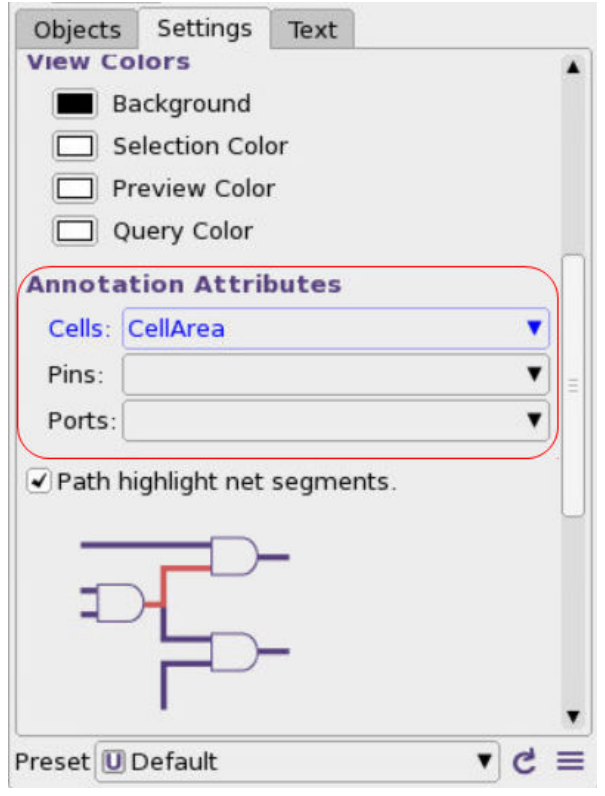
\includegraphics[width=0.8\textwidth]{gui-fig-121.png}
\caption{Settings 页中的 Annotation Attributes}
\label{fig:gui-121}
\end{figure}

图~\ref{fig:gui-122} 中，属性标注为白色：单元上标注 area，管脚上标注 port\_type。

\begin{figure}[htbp]
\centering
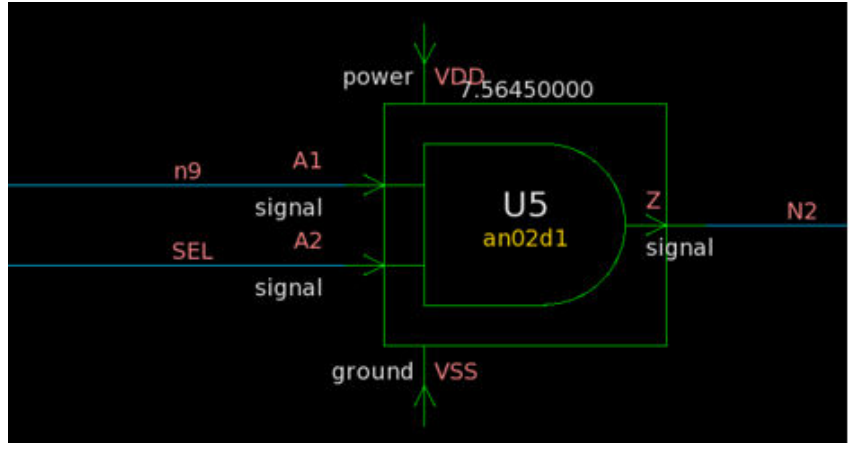
\includegraphics[width=0.8\textwidth]{gui-fig-122.png}
\caption{单元与管脚上的属性标注}
\label{fig:gui-122}
\end{figure}

可以用它调试时序违例，例如在路径管脚上标注 \cmd{late\_rise\_transtion}；也可以分析功耗，例如在路径管脚上标注 \cmd{switching\_activity} 或 \cmd{toggle\_rate}。

\section{在原理图上添加管脚标记}
\subsection*{Adding Pin Markers to the Schematic View}

可以在原理图管脚上加标记，以突出内容。标记可选：
\begin{itemize}
  \item 形状：菱形（diamond）或圆点（dot）；
  \item 颜色：黄、橙或红。
\end{itemize}

右键单击管脚，选择 \textbf{Pin Markers > Set > }\textit{marker\_type}。\textit{marker\_type} 为 Yellow Diamond、Orange Diamond、Red Diamond、Yellow Dot、Orange Dot 或 Red Dot 之一。界面见图~\ref{fig:gui-123}。

\begin{figure}[htbp]
\centering
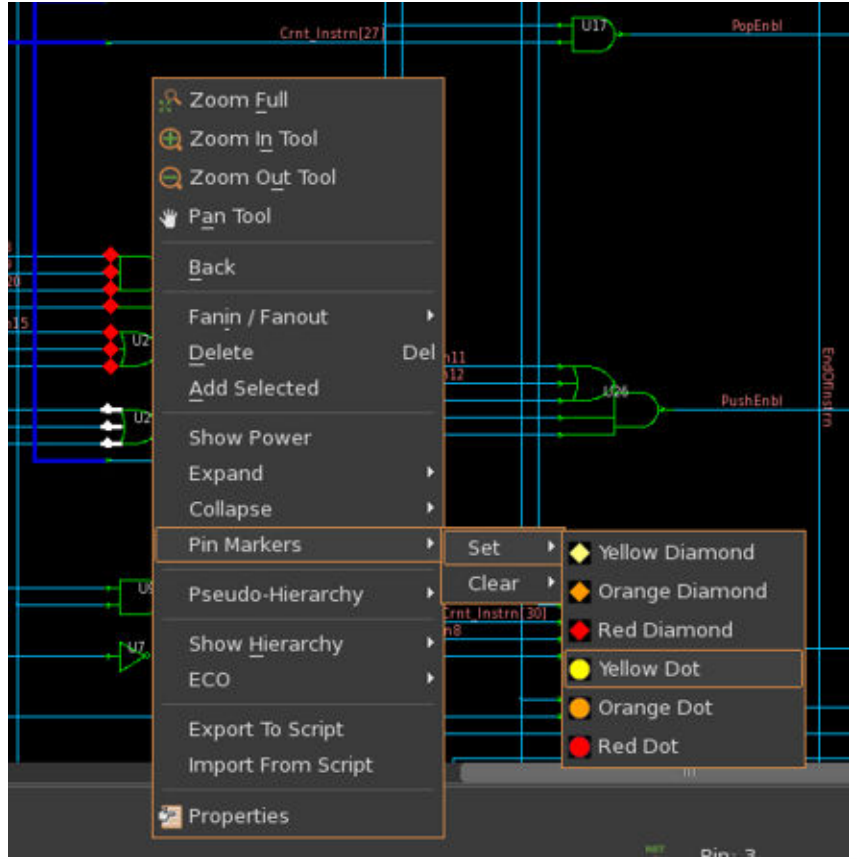
\includegraphics[width=0.7\textwidth]{gui-fig-123.png}
\caption{添加管脚标记}
\label{fig:gui-123}
\end{figure}
